\documentclass{article}
\usepackage{pgfplots}
\usetikzlibrary{pgfplots.groupplots}
\pgfplotsset{compat=1.7}


\begin{document}
	\thispagestyle{empty}

	\begin{figure}[t]
		\centering
		
		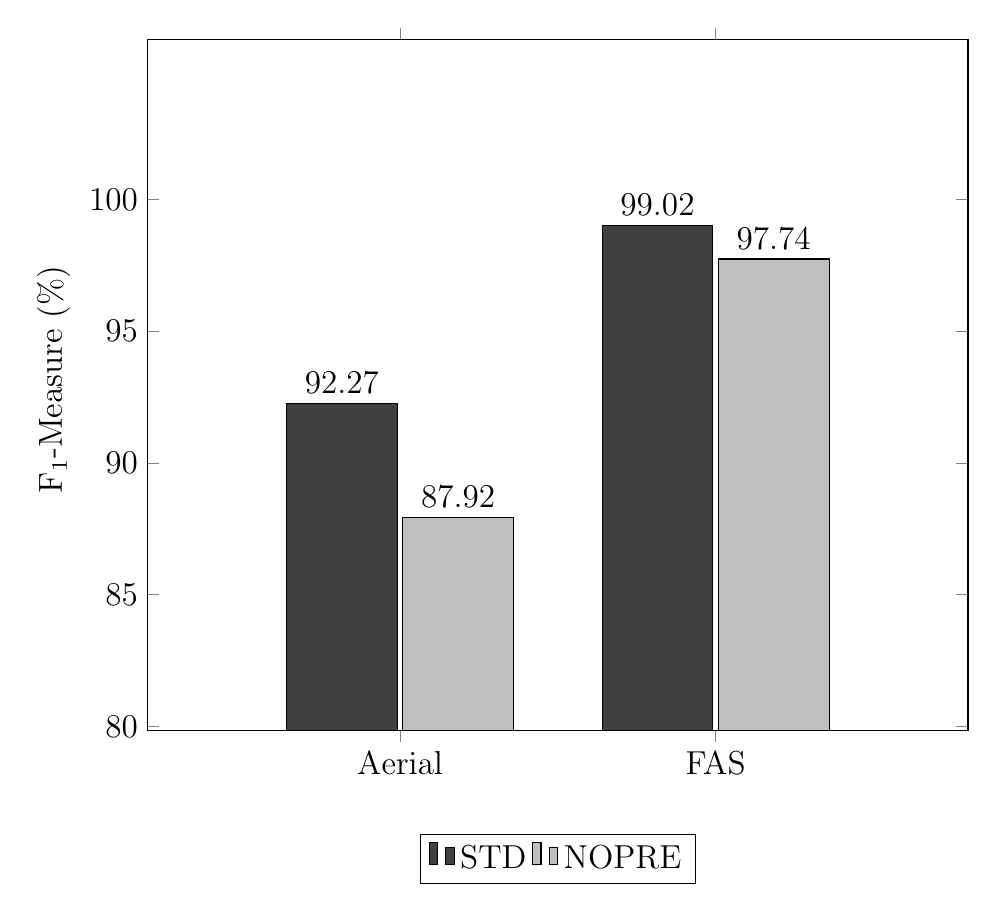
\begin{tikzpicture}
		\begin{axis}[
		width=12cm,
		ybar,
		enlargelimits=0.80,
		legend style={at={(0.5,-0.15)},
			anchor=north,legend columns=-1},
		ylabel={\ F$_1$-Measure (\%)},
		symbolic x coords={Aerial,FAS},
		xtick=data,
		nodes near coords,
		nodes near coords align={vertical},
		bar width=40pt,
		style={font=\large},
		ytick={80,85,...,100},
		ymax=98
		]
%						STD		NPRE
%			Aerial
%				Clean	92,27	87,92
%				Noisy   75,75   80,20

%			FAS		
%				Clean	99,02	97,74
%				Noisy   90,17	89,67

			
		\addplot [color=black,fill=darkgray] coordinates {(Aerial,92.27) (FAS,99.02) };
		\addplot [color=black,fill=lightgray] coordinates {(Aerial,87.92) (FAS,97.74) };

		
		\legend{STD,NOPRE}
		\end{axis}
		\end{tikzpicture}
		%\vspace{-0.7cm}
		%\caption{Left: the pitch distribution for the 10 male speakers. Right: the active speech level for the 20 speakers.}\label{fig:pitch}
		%\vspace{-0.5cm}
	\end{figure}


\end{document}